\section{Current System Architecture}
Figure \ref{fig:system} separates production v3.3 from legacy reference scores and independent context evidence. The unpromoted v3.4 candidate uses the same network.
\begin{figure}[htbp]\centering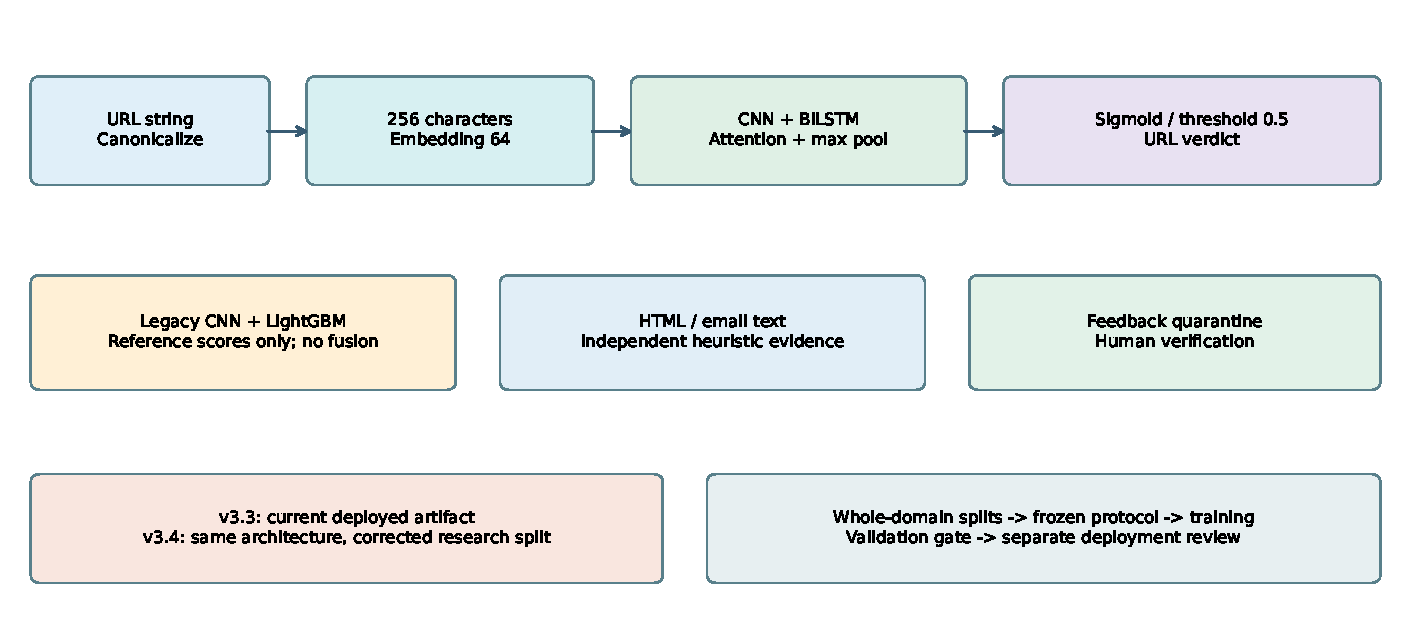
\includegraphics[width=.90\textwidth]{images/system_architecture.pdf}\caption{Versioned classifier and independent extensions}\label{fig:system}\end{figure}

\section{CNN--BiLSTM--Attention Network}
Character indices enter a 64-dimensional embedding. Parallel kernels 3, 5 and 7 each have 128 convolutional channels, BatchNorm and ReLU. Their 384 concatenated channels are max-pooled by two, producing 128 time steps from 256 input positions. Dropout 0.2 precedes the recurrent component. The LSTM has two layers, input width 384, hidden width 128 per direction and a true bidirectional flag. Its output width is 256 at each time step.

Additive attention maps 256 values to 64 and then one score, applies tanh and a time-axis softmax, and computes a weighted sum. This 256-vector is concatenated with a temporal maximum to form 512 values. The classifier has widths 512, 128, 32 and 1, LayerNorm, ReLU, dropout 0.3/0.15 and final sigmoid. There are 1,138,434 parameters. It is not multi-head transformer attention and does not mask padding explicitly.
\begin{figure}[htbp]\centering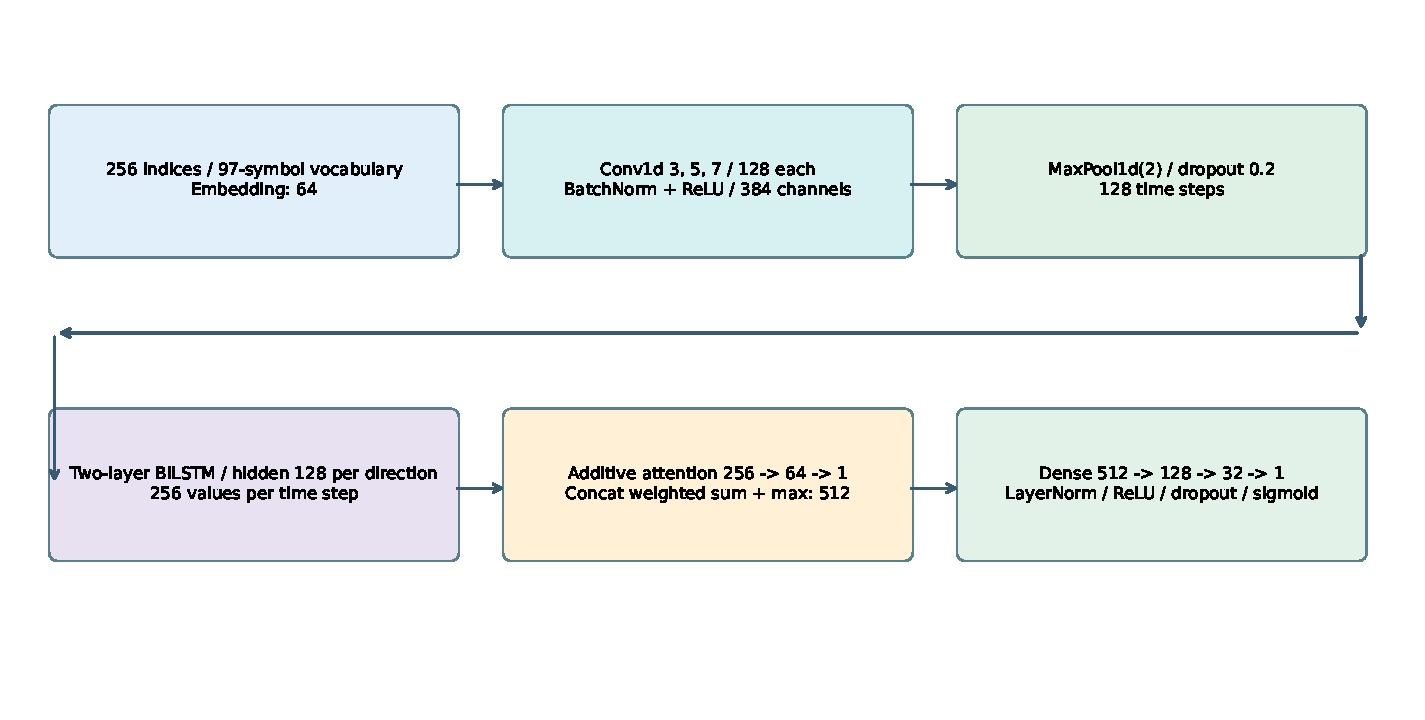
\includegraphics[width=\textwidth]{images/new_model_architecture.pdf}\caption{Exact implemented recurrent architecture}\end{figure}

The original CNN summarized local character patterns with global pooling. The new network retains a sequence of CNN features and reads it in both directions before aggregation. This can model relationships among hostname, path and other character patterns. The theoretical capability does not establish a measured improvement from bidirectionality alone: data, encoding and training exposure also changed between project versions.

\section{Ensemble History}
The reference mixture weights CNN and LightGBM at 60/40. The first independent experiment selected 95/5 on validation AUC. Production V2 later used separately trained artifacts at 35/65. In current production, these component outputs are returned as reference values, while the recurrent probability determines the verdict. The current neural model is therefore not described as a newly calibrated CNN--LightGBM ensemble.

\section{Safe Context and Reviewed Adaptation}
HTML parsing detects structural evidence such as forms, passwords, script/iframe tags, redirect metadata and credential terms. Standalone HTML has no base URL; an absolute target is not proof of cross-origin theft. Email analysis recognizes implemented risk phrases, credential requests, calls to action and URL strings. Neither tool executes code or accesses a mailbox. Both return qualitative evidence rather than validated ML confidence.

Feedback enters quarantine and requires human verification. An approved dataset can feed an explicitly invoked candidate-training process, followed by validation and model versioning. PSI monitors engineered-feature distributions; it does not itself prove an attack or model failure. The project has infrastructure for controlled adaptation, not demonstrated autonomous online learning.